% --------------------------------------------------------------
%                         Preamble
% --------------------------------------------------------------

\documentclass[12pt, letter]{article}
\usepackage[latin1]{inputenc}
\usepackage[T1]{fontenc}
\usepackage{amsmath,amssymb,amsthm}
\usepackage{longtable}
\usepackage{enumitem}
\usepackage{hyperref}
\usepackage{verbatim}
\usepackage{bm}
\usepackage[framemethod=tikz]{mdframed}
\usepackage{graphicx}
\usepackage{amsmath}
\hypersetup{
    colorlinks=true,
    linkcolor=blue,
    filecolor=magenta,      
    urlcolor=blue,
}
 
\urlstyle{same}

\usepackage{array}
\newcolumntype{L}[1]{>{\raggedright\let\newline\\\arraybackslash\hspace{0pt}}m{#1}}
\newcolumntype{C}[1]{>{\centering\let\newline\\\arraybackslash\hspace{0pt}}m{#1}}
\newcolumntype{R}[1]{>{\raggedleft\let\newline\\\arraybackslash\hspace{0pt}}m{#1}}
\newcommand{\norm}[1]{\left\lVert#1\right\rVert}
\newcommand{\vs}[1][1]{\vspace{#1\baselineskip}}

\DeclareMathOperator{\depth}{depth}
\DeclareMathOperator{\im}{im}
\DeclareMathOperator{\coker}{coker}
\DeclareMathOperator{\rank}{rank}
\DeclareMathOperator{\Proj}{Proj}
\DeclareMathOperator{\Hom}{Hom}
\DeclareMathOperator{\Tor}{Tor}
\DeclareMathOperator{\Ext}{Ext}
\DeclareMathOperator{\HH}{H}

% page format

\topmargin -15mm \textwidth 168mm \textheight 240mm \oddsidemargin
-8mm \evensidemargin 0mm
\setlength{\parindent}{0pt}

% some environments :

\theoremstyle{plain}
\newtheorem{theorem}{Theorem}
\newtheorem{lemma}[theorem]{Lemma}
\newtheorem{corollary}[theorem]{Corollary}
\newtheorem{proposition}[theorem]{Proposition}

\numberwithin{theorem}{section}

\theoremstyle{definition}
\newtheorem{definition}[theorem]{Definition}
\newtheorem{example}[theorem]{Example}
\newtheorem{problem}[theorem]{Problem}
\newtheorem{exercise}[theorem]{Exercise}
\newtheorem{algorithm}[theorem]{Algorithm}
\newtheorem{note}[theorem]{Note}
\newtheorem{remark}[theorem]{Remark}
\newtheorem{question}[theorem]{Question}

% using AMS mathematical symbols

\usepackage{latexsym}            % for the qed symbol
\usepackage{amssymb}

\newcommand{\N}{\mathbb{N}}
\newcommand{\Z}{\mathbb{Z}}
\newcommand{\Q}{\mathbb{Q}}
\newcommand{\R}{\mathbb{R}}

\def\qex{\hfill \quad\vrule height1.2ex width0.5em depth 0pt} % end of example


\begin{document}

% --------------------------------------------------------------
%                         Start here
% --------------------------------------------------------------

\noindent
Colorado State University \hfill Section 5 (4:00-4:50pm)\\
Department of Mathematics\ \  \hfill  Math 261, Fall 2019\\
\bigskip
\thispagestyle{empty}

\begin{center}
\begin{large}
\textbf{Lecture Notes-Midterm 2\\
}
\end{large}
\end{center}

% --------------------------------------------------------------
%                         Intro
% --------------------------------------------------------------

\noindent These notes were created by Scott Ziegler for Math 261 at Colorado State University and adapted from Thomas' Calculus, 13th Edition, Pearson Education Inc, 2010. The listed section numbers correspond to the sections of the aforementioned text.


% --------------------------------------------------------------
%                         Sec 14.1
% --------------------------------------------------------------

\section{Functions of Several Variables (14.1)}

We have seen functions of a single variable which map either to a number or a vector. We will now look at the very important concept of functions which take in more than one variable. We'll first look at functions that take in several variables and map them to a real number. Fortunately, our intuition from calc 1 and 2 will serve us very well.

\bigskip

\begin{definition}
Suppose $D$ is a set of $n$-tuples of real numbers $(x_1,x_2,...,x_n)$. A \textbf{real-valued function} $f$ on $D$ is a rule that assigns a unique (single) real number $w=f(x_1,x_2,...,x_n)$ to each element in $D$. The set $D$ is the function's \textbf{domain}. The set of $w$-values taken on by $f$ is the functions's \textbf{range}. The symbol $w$ is the \textbf{dependent variable} of $f$, and $f$ is said to be a function of the $n$ \textbf{independent variables} $x_1$ to $x_n$. We also call the $x_j$'s the function's \textbf{input variables} and call $w$ the function's \textbf{output variable}.
\end{definition}

\bigskip

\hrulefill

\bigskip

\begin{example}
State the domain and range for the following functions of two variables.\\

\smallskip

\begin{itemize}
\item[1.] $z= \sqrt{y-x^2}$. The domain here is all $x,y$ real numbers that satisfy $y\geq x^2$. This produces the range $[0,\infty)$.
\item[2.] $z=\frac{1}{xy}$. The domain here is all $x,y$ real numbers that satisfy $xy\neq 0$. This produces the range $(-\infty, 0) \cup (0,\infty)$.
\item[3.] $z=\sin(xy)$. The domain here is all $x,y$ real numbers. The range here is $[-1,1]$.
\end{itemize}
\end{example}

\bigskip

\hrulefill

\bigskip

\begin{example}
State the domain and range for the following functions of three variables.\\

\smallskip

\begin{itemize}
\item[1.] $w= \sqrt{x^2+y^2+z^2}$. The domain here is all $x,y,z$ real numbers and the range is $[0,\infty)$.
\item[2.] $w=\frac{1}{x^2+y^2+z^2}$. The domain here is all $x,y,z$ real numbers that satisfy $(x,y,z)\neq (0,0,0)$. This produces the range $(0,\infty)$.
\item[3.] $w=xy\ln(z)$.The domain here is all $x,y,z$ real numbers such that $z>0$. The range here is $(-\infty,\infty)$.
\end{itemize}
\end{example}

\bigskip

\hrulefill

\bigskip

\begin{definition}
A point $(x_0,y_0)$ in a region (set) $R$ in the $xy$-plane is an \textbf{interior point} of $R$ if it is the center of a disk of positive radius that lies entirely in $R$. A point $(x_0,y_0)$ is a \textbf{boundary point} of $R$ is every disk centered at $(x_0,y_0)$ contains points that lie outside of $R$ as well as points that lie in $R$. (The boundary point itself need not belong to $R$). The interior points of a region, as a set, make up the \textbf{interior} of the region. The region's boundary points make up its \textbf{boundary}. A region is \textbf{open} if it consists entirely of interior points. A region is \textbf{closed} if it contains all its boundary points.
\end{definition}

\bigskip

\begin{center}
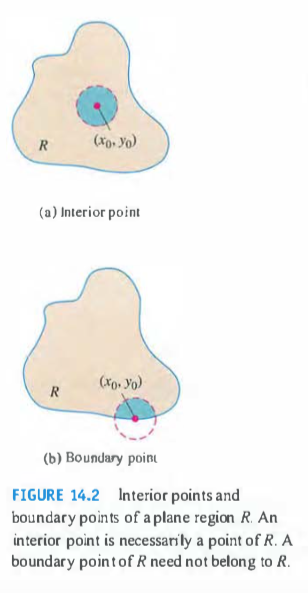
\includegraphics[scale=0.7]{m2_f1}
\end{center}

\bigskip

\textbf{Note:} Just like in 1D, some sets can be neither open nor closed. If you add some boundary points to an open set, it becomes neither open nor closed. There are also sets that are both open and closed!

\bigskip

\hrulefill

\bigskip

\begin{definition}
A region in the plane is \textbf{bounded} if it lies inside a disk of a fixed radius. A region is \textbf{unbounded} if it is not bounded.
\end{definition}

\bigskip

\hrulefill

\bigskip

\begin{example}
Look back to the first example we did today. Is the domain of the function we found open, closed, neither? What about bounded or unbounded? Draw the domain.

\smallskip

\begin{itemize}
\item For $z=\sqrt{y-x^2}$ we found the domain to be $y\geq x^2$. This is the closed, unbounded region above and including the parabola $y=x^2$.
\end{itemize}
\end{example}

\bigskip

\hrulefill

\bigskip

For a function of two variables, we can sketch it by either drawing the surface $z=f(x,y)$ in space of by drawing the level curves (or level sets) of the function.

\bigskip

\begin{definition}
The set of points in the plane where a function $f(x,y)$ has a constant value $f(x,y) = c$ is called a \textbf{level curve} of $f$. The set of all points $(x,y,f(x,y))$ in space, for $(x,y)$ in the domain of $f$, is called the \textbf{graph} of $f$. The graph of $f$ is also called the \textbf{surface} $z=f(x,y)$.

\end{definition}

\bigskip

\hrulefill

\bigskip

\begin{example}
Sketch the graph of $f(x,y) = 100-x^2-y^2$ and plot the level curves $f(x,y) = 0$, $f(x,y) = 51$ and $f(x,y) = 75$ in the domain of $f$ in the plane.

\smallskip

The domain here is the $xy$-plane and the range is all real numbers less than or equal to $100$. The positive portion of the graph is shown below.

\bigskip

\begin{center}
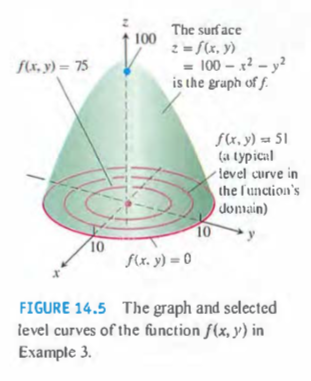
\includegraphics[scale=0.7]{m2_f2}
\end{center}

\bigskip

To find the level sets, note that $f(xy) = 100-x^2-y^2 = 0 \Rightarrow x^2+y^2 = 100$, which is the circle of radius 10 centered at the origin. Similarly we could find the other two level curves to be $x^2+y^2=49$ and $x^2+y^2=25$ and add their plots to the graph.
\end{example}

\bigskip

\hrulefill

\bigskip

For functions of three variables, we can obviously not sketch the graph! However, we could still get some idea of what is going on by sketching the \textbf{level surface} (set of all points $(x,y,z)$ such that $f(x,y,z) = c$). In this case however the level sets are now three dimensional, since the domain of a function of three variables is three dimensional. As an example, describe the level surfaces of the function $f(x,y,z) = \sqrt{x^2+y^2+z^2}$.

\newpage

% --------------------------------------------------------------
%                         Sec 14.2
% --------------------------------------------------------------

\section{Limits and Continuity in Higher Dimensions (14.2)}

We will now talk about limits and continuity in higher dimensions. Most of the definitions you'll see below will look very similar to what you saw in Calc I, with a couple of notable differences.

\bigskip

\begin{definition}
We say that a function $f(x,y)$ approaches the \textbf{limit} $L$ as $(x,y)$ approaches $(x_0,y_0)$, and write
\begin{align*}
\lim_{(x,y) \to (x_0,y_0)} f(x,y) = L
\end{align*}
if, for every number $\epsilon > 0$, there exists a corresponding $\delta > 0$ such that for all $(x,y)$ in the domain of $f$,
\begin{align*}
|f(x,y) - L| < \epsilon \ \ \text{whenever} \ \ 0<\sqrt{(x-x_0)^2+(y-y_0)^2} < \delta.
\end{align*}
\end{definition}

\bigskip

\textbf{Notes:}
\begin{itemize}
\item You won't really ever have to use this definition in this class, but you should note how similar it is to the definition for limits of functions in one dimension!
\item In more plain english, this definition says that the limit of a function at a point $(x_0,y_0)$ exists if for all points $(x,y)$ in the domain of $f$ sufficiently close to $(x_0,y_0)$, the distance between $f(x,y)$ and $L$ is arbitrarily small.
\end{itemize}

\bigskip

All of our rules for limits we had from Calc I still apply here. That is, we still have the sum rule, difference rule, etc.

\bigskip

\hrulefill

\bigskip

\begin{example}
Find the limits indicated for the following functions.

\smallskip

\begin{itemize}
\item $\lim_{(x,y) \to (0,1)} \frac{x-xy+3}{x^2y+5xy-y^3} = \frac{0-(0)(1)+3}{(0)^2(1)+5(0)(1)-(1)^3}
=-3$
\item $\lim_{(x,y) \to ((3,-4)} \sqrt{x^2+y^2} = \sqrt{(3)^2+(-4)^2}
=\sqrt{25} = 5$.
\end{itemize}
\end{example}

\bigskip

\hrulefill

\bigskip

\begin{example}
Find 
\begin{align*}
\lim_{(x,y)\to (0,0)} \frac{x^2-xy}{\sqrt{x}-\sqrt{y}}
\end{align*}

\smallskip

We cannot just ``plug in" our limit value here, we'll have to do a little work. Note that
\begin{align*}
\lim_{(x,y)\to (0,0)} \frac{x^2-xy}{\sqrt{x}-\sqrt{y}} &= \lim_{(x,y) \to (0,0)} \frac{(x^2-xy)(\sqrt{x}+\sqrt{y})}{(\sqrt{x}-\sqrt{y})(\sqrt{x}+\sqrt{y})}\\
&=\lim_{(x,y)\to (0,0)} \frac{x(x-y)(\sqrt{x}+\sqrt{y})}{x-y}\\
&=\lim_{(x,y) \to (0,0)} x(\sqrt{x}+\sqrt{y})\\
&= 0.
\end{align*}
We can cancel $(x-y)$ above because the path $y=x$ is not in the domain of the function (meaning $x-y \neq 0$).
\end{example}

\bigskip

An important note here is that \textit{there is no L'Hospital's Rule for functions of multiple variables}. We can only use algebraic manipulations to help us.

\bigskip

\hrulefill

\bigskip

For functions of one dimension we know that the limit exists if and only if the limit from the left is equal to the limit from the right. There is an analogous idea for functions of two (or more) variables, but it is slightly more complex. We can no longer worry about the limit from only the left and right being equal, but we must instead require that the limit from \textit{every} path approaching the point in question being equal (draw a picture here to help). This leads to the following ``test'.

\bigskip

\begin{proposition}{\textrm{(Two-Path Test for Nonexistence of a Limit)}}
If a function $f(x,y)$ has different limits along two different paths in the domain of $f$ as $(x,y)$ approaches $(x_0,y_0)$, then $\lim_{(x,y)\to (x_0,y_0)} f(x,y)$ does not exist.
\end{proposition}

\bigskip

\hrulefill

\bigskip

\begin{example}
Show that the function
\begin{align*}
f(x,y) = \frac{2x^2y}{x^4+y^2}
\end{align*}
has no limit as $(x,y)$ approaches $(0,0)$.

\smallskip

Along the curve $y=kx^2$ the function has the constant value given by
\begin{align*}
f(x,y) \rvert_{y=kx^2} &= \frac{2x^2y}{x^4+y^2} \rvert_{y=kx^2}\\
&= \frac{2x^2(kx^2)}{x^4+(kx^2)^2}\\
&= \frac{2kx^4}{x^4+k^2x^4}\\
&= \frac{2k}{1+k^2}.
\end{align*}
This means
\begin{align*}
\lim_{(x,y) \to (0,0)_{\text{along} \ y=kx^2}} f(x,y) = \frac{2k}{1+k^2}
\end{align*}
which obviously varies as $k$ varies. Thus by the two-path test we conclude that $f$ has no limit as $(x,y)$ approaches $(0,0)$.
\end{example}

\bigskip

\hrulefill

\bigskip

\begin{example}
If $f(x,y) = \frac{y-2}{x+1}$, does $\lim_{(x,y) \to (-1,2)} f(x,y)$ exist?

\smallskip

If this limit exists then the value of the limit should be the same along any path approaching $(-1,2)$. Notice that along the line $y=2$ the value of the function is $f(x,2) = 0$ for all $x\neq -1$. So if the limit does exist then the value of the limit must be $L=0$. But now consider taking the path given by $y=x+3$. In this case we have $f(x,y) = f(x,x+3) = \frac{x+3-2}{x+1} = \frac{x+1}{x+1} = 1$ for all $x\neq =-1$. By the two path test for nonexistence of a limit, this means that the limit does not exist.
\end{example}

\bigskip

\hrulefill

\bigskip

\begin{definition}
A function $f(x,y)$ is \textbf{continuous at the point} $(x_0,y_0)$ if
\begin{itemize}
\item $f$ is defined at $(x_0,y_0)$,
\item $\lim_{(x,y) \to (x_0,y_0)} f(x,y)$ exists,
\item $\lim_{(x,y) \to (x_0,y_0)} f(x,y) = f(x_0,y_0)$.
\end{itemize}
A function is \textbf{continuous} if it is continuous at every point of its domain.
\end{definition}

\bigskip

This should look almost identical to continuity of functions of one variable. A lot of useful properties of continuous functions in one dimension transfer over well here. That is, the composition of two continuous functions is continuous, there is an extreme value theorem for functions of multiple variables, etc.

\bigskip

\hrulefill

\bigskip

\begin{example}
Is the function given by
\begin{align*}
f(x,y) = \begin{cases} x^2 + y^2, \ (x,y) \neq (0,0) \\ 1, \ (x,y) = (0,0) \end{cases}
\end{align*}
continuous? If not, how could be make it continuous?

\smallskip

No, the function is not continuous at $(x,y) = (0,0)$ as $\lim_{(x,y) \to (0,0)} f(x,y) = 0$ but $f(0,0) = 1$. The easiest fix to make this continuous would be to let $f(0,0) = 0$.
\end{example}

\bigskip

\hrulefill

\bigskip

One last note is that the definitions for limits and thus continuity extend to functions of three or more variables.

\newpage

% --------------------------------------------------------------
%                         Sec 14.3
% --------------------------------------------------------------

\section{Partial Derivatives (14.3)}

It turns out the differentiability for functions of multiple variables is a rather delicate subject. We will not actually define differentiability in this class, but we will discuss the concept of partial derivatives and their relation to differentiability. We'll also practice finding partial derivatives, which should be great news for all of the Calc I lovers out there.

\bigskip

\begin{definition}
The \textbf{partial derivative of} $f(x,y)$ \textbf{with respect to} $x$ at the point $(x_0,y_0)$ is
\begin{align*}
\frac{\partial f}{\partial x} \bigg\rvert_{(x_0,y_0)} = \lim_{h\to 0} \frac{f(x_0+h,y_0)-f(x_0,y_0)}{h},
\end{align*}
provided the limit exists.
\end{definition}

\bigskip

What we're doing in this partial derivative is holding the value of $y$ constant and treating the curve $z=f(x,y_0)$ as only a function of $x$. A good way to visualize this is that we ``cut" the surface $z$ by the plane $y=y_0$. Then if we only look at the surface restricted to that plane, it just looks like a function of one variable! (Draw the picture below if you can or visualize this with a piece of paper to help).

\bigskip

\begin{center}
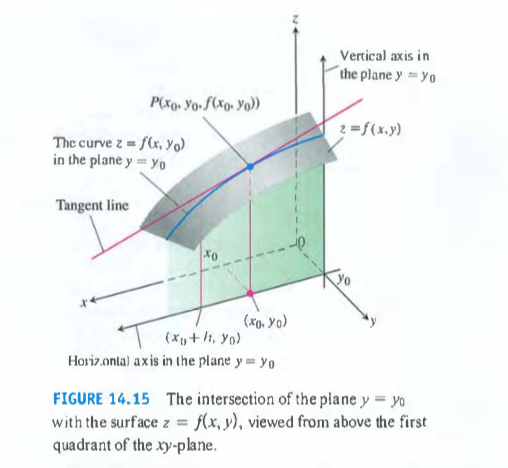
\includegraphics[scale=0.7]{m2_f3}
\end{center}

\bigskip

There is a lot of notation for these partial derivatives, all of the following mean the same thing.
\begin{align*}
\frac{\partial f}{\partial x} (x_0,y_0), \ f_x(x_0,y_0), \ \frac{\partial z}{\partial x}\bigg\rvert_{(x_0,y_0)}
\end{align*}

\bigskip

\hrulefill

\bigskip

\begin{definition}
The \textbf{partial derivative of} $f(x,y)$ \textbf{with respect to} $y$ at the point $(x_0,y_0)$ is
\begin{align*}
\frac{\partial f}{\partial y} \bigg\rvert_{(x_0,y_0)} = \lim_{h\to 0} \frac{f(x_0,y_0+h)-f(x_0,y_0)}{h},
\end{align*}
provided the limit exists.
\end{definition}

\bigskip

The same thing is happening here except that now we are holding $x$ constant!

\bigskip

\begin{center}
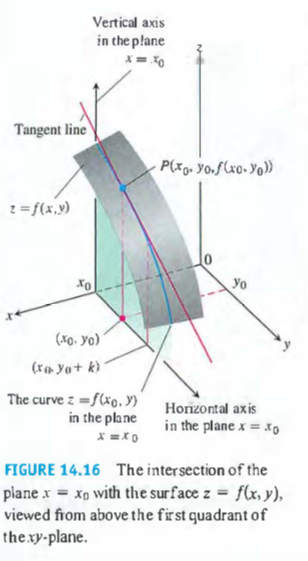
\includegraphics[scale=0.7]{m2_f4}
\end{center}

\bigskip

Notice that now have two tangent lines associated with the surface $z=f(x,y)$. There are an infinite number of tangent lines we could consider, but these two play a special role. Fortunately, these partial derivatives are fairly easy to calculate. All of our rules from Calc I carry over here (product rule, chain rule, quotient rule, implicit differentiation, etc.)

\bigskip

\hrulefill

\bigskip

\begin{example}
Find the values of $\partial f / \partial x$ and $\partial f / \partial y$ at the point $(4,-5)$ if
\begin{align*}
f(x,y) = x^2+3xy+y-1.
\end{align*}
\smallskip

Remember to find each of these partial derivatives we simply keep one of the variables constant and then use our normal derivative rules. So we have
\begin{align*}
\frac{\partial f}{\partial x} &= \frac{\partial}{\partial x} (x^2+3xy+y-1)\\
&=2x+3y+0-0 = 2x+3y
\end{align*}
giving
\begin{align*}
\frac{\partial f}{\partial x}\bigg\rvert_{(4,-5)} = 2(4)+3(-5) = -7.
\end{align*}
For the other partial derivative we get
\begin{align*}
\frac{\partial f}{\partial y} &= \frac{\partial}{\partial y} (x^2+3xy+y-1)\\
&=0+3x+1-0 = 3x+1.
\end{align*}
giving
\begin{align*}
\frac{\partial f}{\partial y}\bigg\rvert_{(4,-5)} = 3(4)+1 = 13.
\end{align*}
\end{example}

\bigskip

\hrulefill

\bigskip

\begin{example}
Find $\partial f / \partial y$ if $f(x,y) = y\sin(xy)$.

\smallskip

Since we are not evaluating anything, our partial derivative here will give us a function. We get
\begin{align*}
\frac{\partial f}{\partial y} &= \frac{\partial}{\partial y} (y\sin(xy)) = y\frac{\partial}{\partial y} \sin(xy) + (\sin(xy))\frac{\partial}{\partial y} (y)\\
&=(y\cos(xy))\frac{\partial}{\partial y}(xy) + \sin(xy) = xy\cos(xy)+\sin(xy).
\end{align*}
\end{example}

\bigskip

\hrulefill

\bigskip

\begin{example}
Find $f_x$ and $f_y$ if
\begin{align*}
f(x,y) = \frac{2y}{y+\cos(x)}
\end{align*}

\smallskip

\begin{align*}
f_x &= \frac{\partial}{\partial x} \left(\frac{2y}{y+\cos(x)}\right) = \frac{(y+\cos(x))\frac{\partial}{\partial x}(2y)-2y\frac{\partial}{\partial x}(y+\cos(x)}{(y+\cos(x))^2})\\
&=\frac{(y+\cos(x))(0)-2y(-\sin(x))}{(y+\cos(x))^2} = \frac{2y\sin(x)}{(y+\cos(x))^2}\\
f_y &= \frac{\partial}{\partial y} \left(\frac{2y}{y+\cos(x)}\right) = \frac{(y+\cos(x))\frac{\partial}{\partial y}(2y)-2y\frac{\partial}{\partial y}(y+\cos(x)}{(y+\cos(x))^2})\\
&=\frac{(y+\cos(x))(2)-2y(1)}{(y+\cos(x))^2} = \frac{2\cos(x)}{(y+\cos(x))^2}\\
\end{align*}
\end{example}

\bigskip

\hrulefill

\bigskip

\begin{example}
Find $\partial z / \partial x$ if the equation
\begin{align*}
yz-\ln(z) = x+y
\end{align*}
defines $z$ a a function of the two independent variables $x$ and $y$ and the partial derivative exists.

\smallskip

We need to use implicit differentiation here, so we will differentiate both sides with respect to $x$ while holding $y$ constant and treating $z$ as a differentiable function of $x$:
\begin{align*}
\frac{\partial}{\partial x} (yz) - \frac{\partial}{\partial x} \ln(z) &= \frac{\partial}{\partial x} x + \frac{\partial y}{\partial x}\\
\Rightarrow y \frac{\partial z}{\partial x} - \frac{1}{z} \frac{\partial z}{\partial x} &= 1+0\\
\Rightarrow \left(y-\frac{1}{z}\right) \frac{\partial z}{\partial x} &= 1\\
\frac{\partial z}{\partial x} &= \frac{z}{yz-1}.
\end{align*}
\end{example}

\bigskip

\hrulefill

\bigskip

All of our derivative rules also carry over to functions of more than two variables.

\bigskip

\hrulefill

\bigskip

\begin{example}
Find $\partial f / \partial z$ where
\begin{align*}
f(x,y,z) = x\sin(y+3z).
\end{align*}
We have
\begin{align*}
\frac{\partial f}{\partial z} &= \frac{\partial}{\partial z}(x\sin(y+3z))\\
&=x \frac{\partial}{\partial z} \sin(y+3z)\\
&=x\cos(y+3z)\frac{\partial}{\partial z}(y+3z)\\
&=3x\cos(y+3z).
\end{align*}
\end{example}

\bigskip

\hrulefill

\bigskip

This is where things start to get a little weird. For functions of one dimension we know that differentiability at a point implies continuity at that point. However, a function of multiple variables can have all of its partial derivatives exist at a point and still not be continuous at that point! Check out the following example.

\bigskip

\hrulefill

\bigskip

\begin{example}
Let
\begin{align*}
f(x,y) = \begin{cases} 0, \ xy\neq 0 \\ 1, \ xy=0 \end{cases}.
\end{align*}
Show that the function is not continuous at $(x,y)=0$, but both partial derivatives $\partial f / \partial x$ and $\partial f / \partial y$ exist at the origin.

\smallskip

The fact that function is not continuous at the origin should be intuitively clear and could be shown with a little work. To see the partial derivatives exist, note that to find $\partial f / \partial x$ at $(0,0)$ we hold $y$ fixed at $y=0$. This means $f(x,y) = 1$ for all $x$, making the partial derivative equal to 0. We could do the same for the other partial derivative, meaning $\partial f / \partial y$ is also equal to 0.
\end{example}

\bigskip

\hrulefill

\bigskip

We're not going to discuss the definition of differentiability in this class. The reason things get complicated is that we can no longer only worry about approaching a point on a function from 2 dimensions, we now have to be concerned with approaching a point from an infinite number of directions! There is one thing we will discuss however.

\bigskip

\begin{theorem}
If the partial derivatives $f_x$ and $f_y$ of a function $f(x,y)$ are continuous throughout an open region $R$, then $f$ is differentiable at every point of $R$.
\end{theorem}

\bigskip

This theorem helps us relate the specific tangent lines associated with $f_x$ and $f_y$ with continuity of the function. Take a look at our funny example above, in that case the partial derivatives were not continuous in any neighborhood around $(0,0)$.

\bigskip

\hrulefill

\bigskip

Just like for functions of one variable, we can discuss higher order partial derivatives for functions of more than one variable. These derivative are denoted as follows.
\begin{align*}
&\frac{\partial^2 f}{\partial x^2} \ \text{or} \ f_{xx}\\
&\frac{\partial^2 f}{\partial y^2} \ \text{or} \ f_{yy}\\
&\frac{\partial^2 f}{\partial x \partial y} \ \text{or} \ f_{yx} \ \text{or} \ (f_y)_x\\
&\frac{\partial^2 f}{\partial y \partial x} \ \text{or} \ f_{xy} \ \text{or} \ (f_x)_y\\
\end{align*}
Notice the order on the ``mixed" partial derivatives!

\bigskip

\hrulefill

\bigskip

\begin{example}
If $f(x,y) = x\cos(y) + ye^x$, find the second-order derivatives
\begin{align*}
\frac{\partial^2 f}{\partial x^2}, \ \frac{\partial^2 f}{\partial y \partial x}, \ \frac{\partial^2 f}{\partial y^2}, \ \text{and} \ \frac{\partial^2 f}{\partial x \partial y}.
\end{align*}

\smallskip

We first need to find both first partial derivatives, which here gives
\begin{align*}
\frac{\partial f}{\partial x} &= \frac{\partial}{\partial x} (x\cos(y)+ye^x)\\
&=\cos(y)+ye^x
\end{align*}
and
\begin{align*}
\frac{\partial f}{\partial y} &= \frac{\partial}{\partial y} (x\cos(y)+ye^x)\\
&=-x\sin(y)+e^x.
\end{align*}
Now our second order partial derivatives are
\begin{align*}
\frac{\partial^2 f}{\partial x^2} &= \frac{\partial}{\partial x} \left(\frac{\partial f}{\partial x}\right) = ye^x\\
\frac{\partial^2 f}{\partial y^2} &= \frac{\partial}{\partial y} \left(\frac{\partial f}{\partial y}\right) = -x\cos(y)\\
\frac{\partial^2 f}{\partial x \partial y} &= \frac{\partial}{\partial x} \left(\frac{\partial f}{\partial y}\right) = -\sin(y)+e^x\\
\frac{\partial^2 f}{\partial y \partial x} &= \frac{\partial}{\partial y} \left(\frac{\partial f}{\partial x}\right) = -\sin(y)+e^x.\\
\end{align*}
\end{example}

\bigskip

\hrulefill

\bigskip

The last example suggests the following.

\bigskip

\begin{theorem}{(The Mixed Derivative Theorem)}
If $f(x,y)$ and its partial derivatives $f_x, f_y, f_{xy}$ and $f_{yx}$ are defined throughout an open region containing a point $(a,b)$ and are all continuous at $(a,b)$, then
\begin{align*}
f_{xy}(a,b) = f_{yx}(a,b).
\end{align*}
\end{theorem}

\bigskip

\hrulefill

\bigskip

It doesn't stop here! We could keep taking partial derivatives of arbitrarily high order (assuming of course that they exist.

\bigskip

\hrulefill

\bigskip

\begin{example}
Find $f_{yxyz}$ if $f(x,y,z) = 1-2xy^2z+x^2y$.

\smallskip

\begin{align*}
f_y &= -4xyz+x^2\\
f_{yx} &= -4yz+2x\\
f_{yxy} &= -4z\\
f_{yxyz} &= -4.
\end{align*}
\end{example}

\newpage

% --------------------------------------------------------------
%                         Sec 14.4
% --------------------------------------------------------------

\section{The Chain Rule (14.4)}

We should be very familiar with the chain rule for functions of a single variable. If $w=f(x)$ is a differentiable function of $x$ and $x=g(t)$ is a differentiable function of $t$, then $w$ is a differentiable function of $t$ and $dw / dt$ can be calculated by
\begin{align*}
\frac{dw}{dt} = \frac{dw}{dx} \frac{dx}{dt}.
\end{align*}
Let's now look at how the chain rule works for functions of multiple variables. Your book splits up the chain rule into a lot of different theorems. We will discuss all of these, but they are all actually just special cases of a more general theorem.

\bigskip

\hrulefill

\bigskip

\begin{theorem}{(Chain Rule for Functions of Two Independent Variables)}
If $w=f(x,y)$ is differentiable and if $x=x(t)$, $y=y(t)$ are differentiable functions of $t$, then the composite $w=f(x(t),y(t))$ is a differentiable function of $t$ and
\begin{align*}
\frac{dw}{dt} = f_x(x(t),y(t)) \cdot x'(t) + f_y(x(t),y(t))\cdot y'(t),
\end{align*}
or,
\begin{align*}
\frac{dw}{dt} = \frac{\partial f}{\partial x} \frac{dx}{dt} + \frac{\partial f}{\partial y} \frac{dy}{dt}.
\end{align*}
\end{theorem}

\bigskip

We will often rewrite the above theorem using slightly different notation:
\begin{align*}
\frac{dw}{dt} = \frac{\partial w}{\partial x} \frac{dx}{dt} + \frac{\partial w}{\partial y} \frac{dy}{dt}.
\end{align*}

\bigskip

The following branch diagram might be a useful tool to remember the chain rule in this case.

\bigskip

\begin{center}
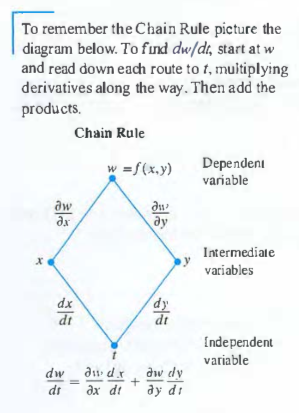
\includegraphics[scale=0.6]{m2_f5}
\end{center}

\bigskip

\hrulefill

\bigskip

\begin{example}
Find the derivative of $w=xy$ with respect to $t$ along the path $x=\cos(t)$, $y=\sin(t)$. What is the derivative's value at $t=\pi/2$?

\smallskip

We can apply the chain rule to get
\begin{align*}
\frac{dw}{dt} &= \frac{\partial w}{\partial x} \frac{dx}{dt} + \frac{\partial w}{\partial y} \frac{dy}{dt}\\
&= \frac{\partial (xy)}{\partial x} \cdot \frac{d}{dt}(\cos(t))+\frac{\partial (xy)}{\partial y} \cdot \frac{d}{dt} (\sin(t))\\
&= y(-\sin(t)) + x(\cos(t))\\
&= -\sin^2(t) + \cos^2(t)\\
&= \cos(2t).
\end{align*}
This gives
\begin{align*}
\frac{dw}{dt} \bigg\rvert_{t=\pi/2} = \cos\left(2\cdot\frac{\pi}{2}\right) = \cos(\pi) = -1.
\end{align*}
\end{example}

\bigskip

\hrulefill

\bigskip

\begin{theorem}{(Chain Rule for Functions of Three Independent Variables)}
If $w=f(x,y,z)$ is differentiable and $x,y$, and $z$ are differentiable functions of $t$, then $w$ is a differentiable function of $t$ and
\begin{align*}
\frac{dw}{dt} = \frac{\partial w}{\partial x} \frac{dx}{dt} + \frac{\partial w}{\partial y} \frac{dy}{dt} + \frac{\partial w}{\partial z} \frac{dz}{dt}.
\end{align*}
\end{theorem}

\bigskip

The branch diagram for this looks like the following.

\bigskip

\begin{center}
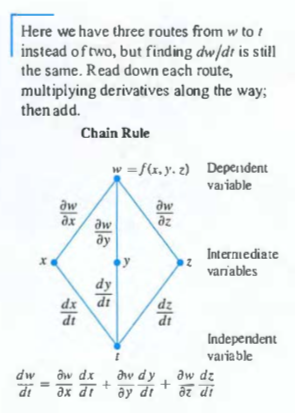
\includegraphics[scale=0.7]{m2_f6}
\end{center}

\bigskip

\hrulefill

\bigskip

\begin{example}
Find $dw/dt$ if $w=xy+z$, $x=\cos(t)$, $y=\sin(t)$, and $z=t$. What is the derivative's value at $t=0$?

\smallskip

We use the chain rule to find
\begin{align*}
\frac{dw}{dt} &= \frac{\partial w}{\partial x} \frac{dx}{dt} + \frac{\partial w}{\partial y} \frac{dy}{dt} + \frac{\partial w}{\partial z} \frac{dz}{dt}\\
&= (y)(-\sin(t))+(x)(\cos(t))+(1)(1)\\
&= -\sin^2(t)+\cos^2(t)+1\\
&= 1+\cos(2t).
\end{align*}
So
\begin{align*}
\frac{dw}{dt} \bigg\rvert_{t=0} = 1+\cos(0) = 2.
\end{align*}
\end{example}

\bigskip

\hrulefill

\bigskip

Let's say now that each of our intermediate variables depend on more than one independent variables. It not longer makes sense to talk about ``regular" derivatives, we now need to look at partial derivatives with respect to each independent variable. This changes the chain rule only slightly.

\bigskip

\begin{theorem}{(Chain Rule for Two Independent Variables and Three Intermediate Variables)}
Suppose that $w=f(x,y,z)$, $x=g(r,s)$, $y=h(r,s)$, and $z=k(r,s)$. If all four functions are differentiable, then $w$ has partial derivatives with respect to $r$ and $s$, given by the formulas
\begin{align*}
\frac{\partial w}{\partial r} &= \frac{\partial w}{\partial x}\frac{\partial x}{\partial r} + \frac{\partial w}{\partial y}\frac{\partial y}{\partial r} + \frac{\partial w}{\partial z}\frac{\partial z}{\partial r}\\
\frac{\partial w}{\partial s} &= \frac{\partial w}{\partial x}\frac{\partial x}{\partial s} + \frac{\partial w}{\partial y}\frac{\partial y}{\partial s} + \frac{\partial w}{\partial z}\frac{\partial z}{\partial s}.
\end{align*}
\end{theorem}

\bigskip

\hrulefill

\bigskip

\begin{example}
Express $\partial w / \partial r$ and $\partial w / \partial s$ in terms of $r$ and $s$ if
\begin{align*}
w=x+2y+z^2, \ x=\frac{r}{s}, \ y=r^2+\ln(s), \ z=2r.
\end{align*}

\smallskip

We can use the chain rule to find these partial derivatives.
\begin{align*}
\frac{\partial w}{\partial r} &= \frac{\partial w}{\partial x} \frac{\partial x}{\partial r} + \frac{\partial w}{\partial y} \frac{\partial y}{\partial r} + \frac{\partial w}{\partial z} \frac{\partial z}{\partial r}\\
&= (1)\left(\frac{1}{s}\right) + (2)(2r)+(2z)(2)\\
&= \frac{1}{s} + 4r+4z\\
&= \frac{1}{s} + 12r.\\
\frac{\partial w}{\partial s} &= \frac{\partial w}{\partial x} \frac{\partial x}{\partial s} + \frac{\partial w}{\partial y} \frac{\partial y}{\partial s} + \frac{\partial w}{\partial z} \frac{\partial z}{\partial s}\\
&= (1)\left(-\frac{r}{s^2}\right) + (2)\left(\frac{1}{s}\right)+(2z)(0)\\
&= \frac{2}{s} - \frac{r}{s^2}.
\end{align*}
\end{example}

\bigskip

\hrulefill

\bigskip

We could of course consider having more or fewer intermediate variables and independent variables in the last theorem, in which case we would have the following.

\bigskip

\begin{theorem}
If $w=f(x,y)$, $x=g(r,s)$, and $y=h(r,s)$, then
\begin{align*}
\frac{\partial w}{\partial r} = \frac{\partial w}{\partial x}\frac{\partial x}{\partial r} + \frac{\partial w}{\partial y}\frac{\partial y}{\partial r} \ \ \text{and} \ \ \frac{\partial w}{\partial s} = \frac{\partial w}{\partial x}\frac{\partial x}{\partial s} + \frac{\partial w}{\partial y}\frac{\partial y}{\partial s}.
\end{align*}
\end{theorem}

\bigskip

\begin{theorem}
If $w=f(x)$ and $x=g(r,s)$, then
\begin{align*}
\frac{\partial w}{\partial r} = \frac{dw}{dx} \frac{\partial x}{\partial r} \ \ \text{and} \ \ \frac{\partial w}{\partial s} = \frac{dw}{dx} \frac{\partial x}{\partial s}
\end{align*}
\end{theorem}

\bigskip

\hrulefill

\bigskip

It turns out the chain rule greatly simplifies the task of implicit differentiation! How? Suppose that we are give the equation
\begin{align*}
F(x,y(x)) = 0
\end{align*}
where $F$ is differentiable and $y$ is a differentiable function of $x$. Then this equation defines $y$ implicitly as a differentiable function of $x$. Now if we take the derivative of both sides of the above equation with respect to $x$, the chain rule gives
\begin{align*}
\frac{d}{dx} F(x,y(x)) &= \frac{d}{dx} 0\\
\Rightarrow F_x \frac{d}{dx}(x) + F_y \frac{dy}{dx} &= 0\\
\Rightarrow F_x + F_y \frac{dy}{dx} &= 0\\
\Rightarrow \frac{dy}{dx} &= -\frac{F_x}{F_y}.
\end{align*} 
This holds at any point for which $F_y \neq 0$.

\bigskip

\hrulefill

\bigskip

\begin{example}
Find $dy/dx$ if $y^2-x^2-\sin(xy) = 0$.

\smallskip

Here we have $F(x,y) = y^2-x^2-\sin(xy)$, so using our above formula gives
\begin{align*}
\frac{dy}{dx} = -\frac{F_x}{F_y} = -\frac{2x-y\cos(xy)}{2y-x\cos(xy)} = \frac{2x+y\cos(xy)}{2y-x\cos(xy)}.
\end{align*}
\end{example}

\bigskip

\hrulefill

\bigskip

You could extend this to functions of multiple variables as well. If we have an equation of the form
\begin{align*}
F(x,y,f(x,y))=0,
\end{align*}
then using the chain rule and proceeding as above would give
\begin{align*}
\frac{\partial z}{\partial x} = -\frac{F_x}{F_z} \ \ \text{and} \ \ \frac{\partial z}{\partial y} = -\frac{F_y}{F_z}.
\end{align*}

\newpage

% --------------------------------------------------------------
%                         Sec 14.5
% --------------------------------------------------------------

\section{Directional Derivatives and Gradient Vectors (14.5)}

Think about the following situation as motivation for this section. You're standing at the top of a mountain and tracking the progress of a stream that moves down the mountain. What direction is the stream taking? Is it meandering downhill, then sideways, then uphill, then back down? No! It's moving directly down the mountain along the paths of steepest descent. What is the relation to the direction in which the stream is moving and the level curves of the mountain?

\bigskip

\begin{definition}
The \textbf{derivative of} $f$ \textbf{at} $P_0(x_0,y_0)$ \textbf{in the direction of the unit vector} $u = u_1 \bm{i} + u_2 \bm{j}$ is the number
\begin{align*}
\left(\frac{df}{ds}\right)_{u,P_0} = \lim_{s\to 0} \frac{f(x_0+su_1, y_0 + su_2) - f(x_0,y_0)}{s},
\end{align*}
provided the limit exists.
\end{definition}

\bigskip

Recall how we find the partial derivatives of the last section. We ``cut" the surface defined by $f(x,y)$ along a plane perpendicular either the $x$ or $y$ axis and looked at the restriction of the surface $f$ to that plane as a function of a single variable. We are doing the same thing here, only we are now cutting the function with a plane that is not necessarily perpendicular to either the $x$ or $y$ axis. (Again use a piece of paper as a visual here). We would use this definition of a directional derivative to produce the definitions we had of a partial derivative. What if we let $\bm{u} = \bm{i}$ or $\bm{u} = \bm{j}$? We get the definition of a partial derviative!

\bigskip

We often denote the directional derivative as $(D_u f)_{P_0}$, read as ``the derivative of $f$ at $P_0$ in the direction of $\bm{u}$.

\bigskip

\hrulefill

\bigskip

Let's see if we can find an easier way to calculate directional derivatives. Start with the line
\begin{align*}
x= x_0+su_1, \ \ \ y= y_0 + su_2
\end{align*}
which runs through $P_0(x_0,y_0)$, is parametrized by the arc length parameter $s$ and runs parallel to the unit vector $\bm{u} = u_1 \bm{i} + u_2 \bm{j}$. Using the chain rule we find the derivative of the function $f(x,y)$ is
\begin{align*}
\left( \frac{df}{ds} \right)_{u,P_0} &= \left(\frac{\partial f}{\partial x} \right)_{P_0} \frac{dx}{ds} + \left(\frac{\partial f}{\partial y} \right)_{P_0} \frac{dy}{ds}\\
&= \left(\frac{\partial f}{\partial x} \right)_{P_0} u_1 + \left(\frac{\partial f}{\partial y} \right)_{P_0} u_2\\
&= \left( \left(\frac{\partial f}{\partial x}\right)_{P_0} \bm{i} + \left(\frac{\partial f}{\partial y} \right)_{P_0} \bm{j} \right) \cdot \left(u_1\bm{i} + u_2 \bm{j}\right).
\end{align*}
The second term above is the direction of $\bm{u}$, and the first term is something called the \textbf{gradient} of $f(x,y)$, which we define below.

\bigskip

\begin{definition}
The \textbf{gradient vector (gradient)} of $f(x,y)$ at a point $P_0(x_0,y_0)$ is the vector
\begin{align*}
\nabla f = \frac{\partial f}{\partial x} \bm{i} + \frac{\partial f}{\partial y} \bm{j}
\end{align*}
obtained by evaluating the partial derivatives of $f$ at $P_0$.
\end{definition}

\bigskip

This leads to the following useful formula

\bigskip

\begin{theorem}
If $f(x,y)$ is differentiable in an open region containing $P_0(x_0,y_0)$, then
\begin{align*}
\left( \frac{df}{ds} \right)_{u,P_0} = \left(\nabla f\right)_{P_0} \cdot \bm{u},
\end{align*}
the dot product of the gradient $\nabla f$ at $P_0$ and $\bm{u}$.
\end{theorem}

\bigskip

\hrulefill

\bigskip

\begin{example}
Find the derivative of $f(x,y) = xe^y + \cos(xy)$ at the point $(2,0)$ in the direction of $v=3\bm{i}-4\bm{j}$.

\smallskip

We first need to find the unit vector pointing in the direction of $v$. This gives
\begin{align*}
\bm{u} &= \frac{\bm{v}}{||\bm{v}||}\\
&= \frac{\bm{v}}{\sqrt{3^2+(-4)^2}}\\
&= \frac{\bm{v}}{5}\\
&= \frac{3}{5}\bm{i} - \frac{4}{5}\bm{j}.
\end{align*}
Now we need to find the gradient of $f$ at $(2,0)$, so see that
\begin{align*}
\nabla f& = \frac{\partial f}{\partial x} \bm{i} + \frac{\partial f}{\partial y} \bm{j}\\
&= (e^y-y\sin(xy))\bm{i} + (xe^y-x\sin(xy))\bm{j}\\
\Rightarrow \nabla f \rvert_{(2,0)} &= \bm{i} + 2\bm{j}.
\end{align*}
So our directional derivative is
\begin{align*}
(D_u f) \rvert_{(2,0)} &= \nabla f \rvert_{(2,0)} \cdot \bm{u}\\
&= \left( \bm{i}  + 2\bm{j} \right) \cdot \left(\frac{3}{5}\bm{i} - \frac{4}{5}\bm{j} \right)\\
&= \frac{3}{5} - \frac{8}{5}\\
&= -1.
\end{align*}
\end{example}

\bigskip

\textbf{Important!} The gradient is a \textit{vector} which lies in the \textbf{domain} of the function. So we can think of the gradient (and $\bm{u}$) as lying ``below" the function.

\bigskip

\hrulefill

\bigskip

If we think of the directional derivative as $D_u f = ||\nabla f|| ||\bm{u}|| \cos(\theta) = ||\nabla f|| \cos(\theta)$ we see some nice properties.
\begin{itemize}
\item[1.] The directional derivative is maximized when $\theta = 0$, meaning the directional derivative points in the direction of the gradient of $f$. This means that at each point $P$ in its domain, $f$ increases most rapidly in the direction of the gradient vector $\nabla f$ at $P$.
\item[2.] The directional derivative is minimized when $\theta = \pi$, meaning the directional derivative points in the opposite direction of the gradient of $f$. This means that at each point $P$ in its domain, $f$ decreases most rapidly in the direction of the  negative gradient vector $\nabla f$ at $P$.
\item[3.] The directional derivative is zero when $\theta = \pi/2$, meaning any vector orthogonal to $\nabla f$ gives a direction of zero change in $f$.
\end{itemize}

\bigskip

\hrulefill

\bigskip

\begin{example}
Find the directions in which $f(x,y) = (x^2/2) + (y^2/2)$
\begin{itemize}
\item[1.] increases most rapidly at the point $(1,1)$.

\smallskip

We know that the function increases most rapidly at $(1,1)$ in the direction of the gradient at that point. The gradient here is
\begin{align*}
\nabla f &= \frac{\partial f}{\partial x}\bm{i} + \frac{\partial f}{\partial y}\bm{j}\\
&= x\bm{i} + y\bm{j}\\
\Rightarrow \nabla f \rvert_{(1,1)} &= \bm{i} + \bm{j}
\end{align*}
which has direction
\begin{align*}
\bm{u} &= \frac{\bm{i}+\bm{j}}{||\bm{i}+\bm{j}||}\\
&= \frac{\bm{i} + \bm{j}}{\sqrt{1^2+1^2}}\\
&= \frac{1}{\sqrt{2}}\bm{i} + \frac{1}{\sqrt{2}}\bm{j}.
\end{align*}

\item[2.] decreases most rapidly at the point $(1,1)$.

\smallskip

We know the function decreases most rapidly in the direction of the negative gradient, so
\begin{align*}
-\bm{u} = -\frac{1}{\sqrt{2}} \bm{i} - \frac{1}{\sqrt{2}} \bm{j}.
\end{align*}

\item[3.] What are the directions of zero change in $f$ at $(1,1)$?

\smallskip

The directions of zero change at $(1,1)$ are all directions orthogonal to $\nabla f$, which here are
\begin{align*}
\bm{n} = -\frac{1}{\sqrt{2}} \bm{i} + \frac{1}{\sqrt{2}} \bm{j} \ \ \text{and} \ \ -\bm{n} = \frac{1}{\sqrt{2}} \bm{i} - \frac{1}{\sqrt{2}} \bm{j}.
\end{align*}
\end{itemize}
\end{example}

\bigskip

\hrulefill

\bigskip

All of these rules generalize to higher dimensions. In three dimensions we have
\begin{align*}
\nabla f = \frac{\partial f}{\partial x} \bm{i} + \frac{\partial f}{\partial y} \bm{j} + \frac{\partial f}{\partial z} \bm{k}
\end{align*}
and
\begin{align*}
D_u f = \nabla f \cdot \bm{u} = \frac{\partial f}{\partial x} u_1 + \frac{\partial f}{\partial y} u_2 + \frac{\partial f}{\partial z} u_3
\end{align*}

\bigskip

\hrulefill

\bigskip

\begin{example}
\begin{itemize}
\item[1.] Find the derivative of $f(x,y,z) = x^3 - xy^2-z$ at $P_0(1,1,0)$ in the direction of $\bm{v} = 2\bm{i} - 3\bm{j} + 6\bm{k}$.

\smallskip

We first need to find the unit vector in the direction of $\bm{v}$.
\begin{align*}
\bm{u} &= \frac{\bm{v}}{||\bm{v}||}\\
&= \frac{\bm{v}}{\sqrt{2^2+(-3)^2+6^2}}\\
&= \frac{\bm{v}}{7}\\
&= \frac{2}{7}\bm{i} - \frac{3}{7}\bm{j} + \frac{6}{7}\bm{k}.
\end{align*}
Our gradient at $(1,1,0)$ is
\begin{align*}
\nabla f &= \frac{\partial f}{\partial x} \bm{i} + \frac{\partial f}{\partial y} \bm{j} + \frac{\partial f}{\partial z} \bm{k}\\
&= (3x^2-y^2)\bm{i} + (-2xy)\bm{j} +(-1)\bm{k}\\
\Rightarrow \nabla f \rvert_{(1,1,0)} &= 2\bm{i} - 2\bm{j} - \bm{k}.
\end{align*}
Which means our directional derivative is
\begin{align*}
(D_u f)_{(1,1,0)} &= \left(2\bm{i} - 2\bm{j} - \bm{k}\right) \cdot \left(\frac{2}{7}\bm{i} - \frac{3}{7}\bm{j} + \frac{6}{7}\bm{k}\right)\\
&= \frac{4}{7} + \frac{6}{7} -\frac{6}{7}\\
&= \frac{4}{7}.
\end{align*}

\item[2.] In what directions does $f$ change most rapidly at $P_0$, and what are the rates of change in these directions?

\smallskip

The function increases most rapidly in the direction of $\nabla f$ and decreases most rapidly in the direction of $-\nabla f$. The rates of change of these directions are
\begin{align*}
||\nabla f|| = \sqrt{(2)^2+(-2)^2+(-1)^2} = 3 \ \ \text{and} \ \ - ||\nabla f|| = -3.
\end{align*}
\end{itemize}
\end{example}

\bigskip

\hrulefill

\bigskip

There is a nice relationship between gradients and tangents to level curves. Take a level curve to $f$ given by $\bm{r} = g(t) \bm{i} + h(t) \bm{j}$, then $f(g(t),h(t)) = c$ and we get the following.
\begin{align*}
\frac{d}{dt} f(g(t),h(t)) &= \frac{d}{dt}(c)\\
\Rightarrow \frac{\partial f}{\partial x} \frac{dg}{dt} + \frac{\partial f}{\partial y} \frac{dh}{dt} &= 0\\
\Rightarrow \left(\frac{\partial f}{\partial x} \bm{i}+\frac{\partial f}{\partial y} \bm{j}\right) \cdot \left(\frac{dg}{dt} \bm{i}+\frac{dh}{dt} \bm{j}\right) &= 0\\
\Rightarrow \nabla f \cdot \frac{d\bm{r}}{dt} &= 0.
\end{align*}

\bigskip

This means that the gradient at a point is always orthogonal to the level curve at that point. This allows us to write tangent lines to level curves using the gradient:
\begin{align*}
f_x(x_0,y_0)(x-x_0) + f_y(x_0,y_0)(y-y_0) = 0
\end{align*}
gives the equation of the line tangent to the level curve at $(x_0,y_0)$.

\bigskip

\hrulefill

\bigskip

\begin{example}
Consider the elliptic paraboloid given by $z=f(x,y)=x^2+y^2$. Draw a few of the level sets for this curve, including the level set corresponding to $z=1$. Now find and plot $\nabla f(1,0), -\nabla f(1,0)$ and the tangent line to the curve at $(1,0)$. What do you notice?

\smallskip

The level curves here are just circles with various radii. To find $\nabla f\rvert_{(1,0)}$ and $-\nabla f\rvert_{(1,0)}$ we use the definition of the gradient to find
\begin{align*}
\nabla f &= \frac{\partial f}{\partial x} \bm{i} + \frac{\partial f}{\partial y} \bm{j}\\
&= 2x \bm{i} + 2y \bm{j}\\
\Rightarrow \nabla f\rvert_{(1,0)} &= 2\bm{i}.
\end{align*}
This means that $-\nabla f \rvert_{(1,0)} = -2\bm{i}$. We can now use what we found above to determine the tangent line at $(1,0)$.
\begin{align*}
2(x-1)+(0)(y-0) &= 0\\
\Rightarrow x &= 1.
\end{align*}
After plotting all of these, we notice that the gradient is normal to the level curve at $(1,0)$ and normal to the tangent line at that point.
\end{example}

\newpage

% --------------------------------------------------------------
%                         Sec 14.6
% --------------------------------------------------------------

\section{Tangent Planes and Linearization (14.6)}

For curves in one dimension, we often discuss tangent lines of those curves. For curves or surfaces in higher dimensions, we will discuss tangent planes to the curves or surfaces. We'll first find tangent planes to level surfaces then discuss tangent planes to graphs of a function.

\bigskip

\begin{definition}
The \textbf{tangent plane} at the point $P_0(x_0,y_0,z_0)$ on the level surface face $f(x,y,z) = c$ of a differentiable function $f$ is the plane through $P_0$ normal to $\nabla f \rvert_{P_0}$.

\smallskip

The \textbf{normal line} of the surface at $P_0$ is the line through $P_0$ parallel to $\nabla f \rvert_{P_0}$.
\end{definition}

\bigskip

(Use a sheet of paper here to describe tangent planes.) We have useful formulas for tangent planes and normal lines.

\bigskip

\begin{definition}
Tangent Plane to $f(x,y,z)=c$ at $P_0(x_0,y_0,z_0)$:
\begin{align*}
f_x(P_0)(x-x_0) + f_y(P_0)(y-y_0) + f_z(P_0)(z-z_0) = 0
\end{align*}
Normal line to $f(x,y,z)=c$ at $P_0(x_0,y_0,z_0)$:
\begin{align*}
x=x_0+f_x(P_0)t, \ \ y=y_0+f_y(P_0)t, \ \ z=z_0+f_z(P_0)t.
\end{align*}
\end{definition}

\bigskip

\hrulefill

\bigskip

\begin{example}
Find the tangent plane and normal line of the surface
\begin{align*}
f(x,y,z) = x^2+y^2+z-9 = 0
\end{align*}
at the point $P_0(1,2,4)$. (Draw a picture).

\bigskip

\begin{center}
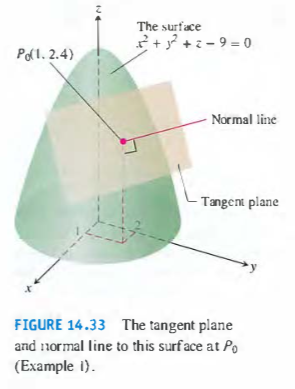
\includegraphics[scale=0.7]{m2_f7}
\end{center}

\bigskip

The tangent plane is the plane through $P_0$ perpendicular to $\nabla f \rvert_{P_0}$. We have
\begin{align*}
\nabla f \rvert_{P_0} = (2x\bm{i} + 2y\bm{j} + \bm{k})_{(1,2,4)} = 2\bm{i} + 4\bm{j} + \bm{k}.
\end{align*}
So our tangent plane is
\begin{align*}
2(x-1)+4(y-2)+(z-4) &= 0 \\
\Rightarrow 2x+4y+z=14.
\end{align*}
The normal line of the surface is then
\begin{align*}
x=1+2t, \ \ y=2+4t, \ \ z=4+t.
\end{align*}

\end{example}

\bigskip

\hrulefill

\bigskip

If we instead want to find tangent planes to the graph of $z=f(x,y)$, note that $z=f(x,y) \Rightarrow f(x,y)-z=0$. So $z=f(x,y)$ is the zero level surface of the function $F(x,y,z) = f(x,y)-z$. Applying our formula above to $F(x,y,z)$ then gives the following formula
\begin{definition}
The plane tangent to the surface $z=f(x,y)$ of a differentiable function $f$ at the point $P_0(x_0,y_0,z_0) = (x_0,y_0,f(x_0,y_0))$ is
\begin{align*}
f_x(x_0,y_0)(x-x_0)+f_y(x_0,y_0)(y-y_0)-(z-z_0) = 0.
\end{align*}
\end{definition}

\bigskip

\hrulefill

\bigskip

\begin{example}
Find the plane tangent to the surface $z=x\cos(y)-ye^x$ at $(0,0,0)$.

\smallskip

Our partial derivatives of $f(x,y) = x\cos(y)-ye^x$ are
\begin{align*}
f_x(x,y) &= \left(\cos(y)-ye^x\right)\\
\Rightarrow f_x(0,0) &= 1-0(1) = 1\\
f_y(x,y) &= \left(-x\sin(y)-e^x\right)\\
\Rightarrow f_y(0,0) &= 0-1 = -1.
\end{align*}
So our tangent plane is
\begin{align*}
1(x-0)-1(y-0)-(z-0) &= 0\\
\Rightarrow x-y-z &= 0.
\end{align*}
\end{example}

\bigskip

\hrulefill

\bigskip

\begin{example}
The surfaces
\begin{align*}
f(x,y,z) = x^2+y^2-2=0
\end{align*}
and
\begin{align*}
g(x,y,z) = x+z-4=0
\end{align*}
meet in an ellipse $E$. (Draw picture).

\bigskip

\begin{center}
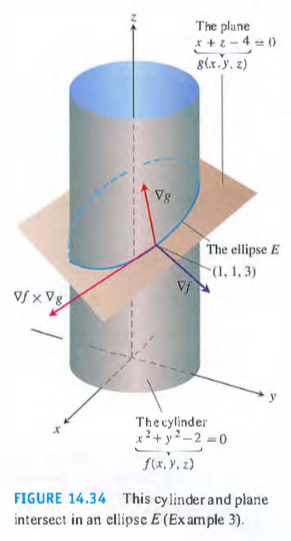
\includegraphics[scale=0.7]{m2_f8}
\end{center}

\bigskip

Find parametric equations for the line tangent to $E$ at the point $P_0(1,1,3)$.

\bigskip

The tangent line is orthogonal to both $\nabla f$ and $\nabla g$ at $P_0$, meaning it is parallel to $\bm{v} = \nabla f \times \nabla g$. Some calculations give
\begin{align*}
\nabla f &= 2x\bm{i}+2y\bm{j}+0\bm{k}\\
\Rightarrow \nabla f \rvert_{(1,1,3)} = 2\bm{i} + 2\bm{j}\\
\nabla g &= \bm{i}+0\bm{j}+\bm{k}\\
\Rightarrow \nabla g \rvert_{(1,1,3)} = \bm{i} + \bm{k}\\
\Rightarrow \bm{v} &= (2\bm{i}+2\bm{j}) \times (\bm{i}+\bm{k})\\
&= \begin{pmatrix} \bm{i} & \bm{j} & \bm{k} \\ 2 & 2 & 0 \\ 1 & 0 & 1 \end{pmatrix}\\
&= 2\bm{i}-2\bm{j}-2\bm{k}.
\end{align*}
So the tangent line is 
\begin{align*}
x=1+2t, \ \ y=1-2t, \ \ z=3-2t.
\end{align*}
\end{example}

\bigskip

\hrulefill

\bigskip

For complicated functions, it is often useful to linearize the function. By this, we mean replace the complicated function with a linear function that is in some way ``close" to the original function.

\bigskip

\begin{definition}
The \textbf{linearization} of a function $f(x,y)$ at a point $(x_0,y_0)$ where $f$ is differentiable is the function
\begin{align*}
L(x,y) = f(x_0,y_0) + f_x(x_0,y_0)(x-x_0) + f_y(x_0,y_0)(y-y_0).
\end{align*}
The approximation
\begin{align*}
f(x,y) \approx L(x,y)
\end{align*}
is the \textbf{standard linear approximation} of $f$ at $(x_0,y_0)$.
\end{definition}

\bigskip

This is actually just the first order Taylor approximation of the function $f$! We'll talk about this more later.

\bigskip

\hrulefill

\bigskip


\begin{example}
Find the linearization of
\begin{align*}
f(x,y) = x^2-xy+\frac{1}{2}y^2+3
\end{align*}
at the point $(3,2)$.

\smallskip

We have
\begin{align*}
f(3,2) &= (3)^2-(3)(2)+\frac{1}{2}(2)^2+3 = 8\\
f_x(x,y) &=2x-y\\
\Rightarrow f_x(3,2) &= 4\\
f_y(x,y) &= -x+y\\
\Rightarrow f_y(3,2) &= -1.
\end{align*}
So our linearization is
\begin{align*}
L(x,y) &= f(3,2) + f_x(3,2)(x-3)+f_y(3,2)(y-2)\\
&= 8+4(x-3)+(-1)(y-2)\\
&=4x-y-2.
\end{align*}
\end{example}

\bigskip

\hrulefill

\bigskip

We may want to know how ``good" the previous approximation is. Fortunately, we can put a bound on the error of the approximation $E(x,y) = f(x,y) - L(x,y)$ that should look familiar.

\bigskip

\begin{definition}
If $f$ has continuous first and second partial derivatives throughout an open set containing a rectangle $R$ centered at $(x_0,y_0)$ and if $M$ is any upper bound for the values of $|f_{xx}|, |f_{yy}|$, and $|f_{xy}|$ on $R$, then the error $E(x,y)$ incurred in replacing $f(x,y)$ by its linearization satisfies the inequality
\begin{align*}
|E(x,y)| \leq \frac{1}{2} M \left(|x-x_0|+|y-y_0|\right)^2.
\end{align*}
\end{definition}

\bigskip

\hrulefill

\bigskip

\begin{example}
Find an upper bound for the approximation in the last example over the rectangle
\begin{align*}
R: \ |x-3| \leq 0.1, \ \ |y-2| \leq 0.1.
\end{align*}

\smallskip

We will use the inequality
\begin{align*}
|E(x,y)| \leq \frac{1}{2} M (|x-x_0|+|y-y_0|)^2.
\end{align*}
To find $M$ we need to know the largest value(s) that one of $f_{xx}, f_{xy}$ and $f_{yy}$ can take in the rectangle. 
\begin{align*}
|f_{xx}| = |2| = 2, \ \ |f_{xy}| = |-1|, \ \ |f_{yy}| = |1| = 1.
\end{align*}
Thus we should take $M=2$, so a bound on our error is
\begin{align*}
|E(x,y)| \leq (|x-x_0|+|y-y_0|)^2
\end{align*}
and since $|x-3| \leq 0.1$ and $|y-2| \leq 0.1$ on $R$, we get
\begin{align*}
|E(x,y)| \leq (0.1+0.1)^2 = 0.04.
\end{align*}
\end{example}

\bigskip

\hrulefill

\bigskip

The facts about linearization and approximation we found for functions of two variables extend to functions of three (or more) variables as well. That is to say, for functions of three variables our linearization is
\begin{align*}
L(x,y,z) = f(x_0,y_0,z_0) + f_x(x_0,y_0,z_0)(x-x_0) + f_y(x_0,y_0,z_0)(y-y_0) + f_z(x_0,y_0,z_0)(z-z_0)
\end{align*}
with error approximation
\begin{align*}
|E(x,y,z)| \leq \frac{1}{2} M \left(|x-x_0|+|y-y_0|+|z-z_0|\right)^2.
\end{align*}


\bigskip

\hrulefill

\bigskip

\begin{example}
Find the linearization of the function
\begin{align*}
f(x,y,z) = x^2-xy+3\sin(z)
\end{align*}
at the point $(x_0,y_0,z_0) = (2,1,0)$.

\smallskip

We have
\begin{align*}
f(2,1,0) &= 2\\
f_x(x,y,z) &= 2x-y\\
\Rightarrow f_x(2,1,0) &= 3\\
f_y(x,y,z) &= -x\\
\Rightarrow f_y(2,1,0) &= -2\\
f_z(x,y,z) &=3\cos(z)\\
\Rightarrow f_z(2,1,0) &= 3\\.
\end{align*}
So our linearization is
\begin{align*}
L(x,y,z) &= 2+3(x-2)+(-2)(y-1)+3(z-0)\\
&= 3x-2y+3z-2.
\end{align*}
\end{example}

\newpage

% --------------------------------------------------------------
%                         Sec 14.7
% --------------------------------------------------------------

\section{Extreme Values and Saddle Points (14.7)}

We're now going to look at how to identify extreme values for functions of two dimensions. It should look very familiar!

\bigskip

\begin{definition}
Let $f(x,y)$ be defined on a region $R$ containing the point $(a,b)$. Then
\begin{itemize}
\item[1.] $f(a,b)$ is a \textbf{local maximum} value of $f$ if $f(a,b) \geq f(x,y)$ for all domain points $(x,y)$ in an open disk centered at $(a,b)$.
\item[2.] $f(a,b)$ is a \textbf{local maximum} value of $f$ if $f(a,b) \leq f(x,y)$ for all domain points $(x,y)$ in an open disk centered at $(a,b)$.
\end{itemize}
\end{definition}

\bigskip

Collectively we refer to the above as local or relative extrema. Just like in one dimension, the key to finding these relative extrema is to use information about the first derivative.

\bigskip

\hrulefill

\bigskip

\begin{theorem}{(First Derivative Test for Local Extreme Values)}
If $f(x,y)$ has a local maximum or minimum value at an interior point $(a,b)$ of its domain and if the first partial derivatives exist there, then $f_x(a,b) = 0$ and $f_y(a,b)=0$.
\end{theorem}

\bigskip

This theorem is equivalent to saying that the surface defined by $z=f(x,y)$ has a horizontal tangent plane at a local extremum (provided the tangent plane exists).

\bigskip

\hrulefill

\bigskip

\begin{definition}
An interior point of the domain of a function $f(x,y)$ where both $f_x$ and $f_y$ are zero or where one or both of $f_x$ and $f_y$ do not exist is a \textbf{critical point} of $f$.
\end{definition}

\bigskip

\hrulefill

\bigskip

This means that the only place that extremum can occur is critical points or boundary points. BUT, a critical point need not be a local extrema.

\bigskip

\begin{definition}
A differentiable function $f(x,y)$ has a \textbf{saddle point} at a critical point $(a,b)$ if in every open disk centered at $(a,b)$ there are domain points $(x,y)$ where $f(x,y) > f(a,b)$ and domain points $(x,y)$ where $f(x,y) < f(a,b)$. The corresponding point $(a,b,f(a,b))$ on the surface $z=f(x,y)$ is called a saddle point of the surface.
\end{definition}

\bigskip

\hrulefill

\bigskip

\begin{example}
Find all critical points of $f(x,y) = x^2+y^2-4y+9$.

\smallskip

Here we have
\begin{align*}
f_x = 2x \ \ \text{and} \ \ f_y = 2y-4.
\end{align*}
So searching for critical points gives
\begin{align*}
f_x &= 2x = 0 \Rightarrow x=0\\
f_y = 2y-4 =0 \Rightarrow y=2.
\end{align*}
So our only critical point is $(0,2)$.
\end{example}

\bigskip

\hrulefill

\bigskip

\begin{example}
Find all critical points of $f(x,y) = y^2-x^2$.

\smallskip

Here we have
\begin{align*}
f_x = -2x \ \ \text{and} \ \ f_y = 2y.
\end{align*}
So searching for critical points gives
\begin{align*}
f_x &= -2x = 0 \Rightarrow x=0\\
f_y = 2y =0 \Rightarrow y=0.
\end{align*}
So our only critical point is $(0,0)$.
\end{example}

\bigskip

\hrulefill

\bigskip

\begin{theorem}{(Second Derivative Test for Local Extreme Values)}
Suppose that $f(x,y)$ and its first and second partial derivatives are continuous throughout a disk centered at $(a,b)$ and that $f_x(a,b) = f_y(a,b)=0$. Then
\begin{itemize}
\item[1.] $f$ has a \textbf{local maximum} at $(a,b)$ if $f_{xx} <0$ and $f_{xx}f_{yy}-f_{xy}^2>0$ at $(a,b)$.
\item[2.] $f$ has a \textbf{local minimum} at $(a,b)$ if $f_{xx} >0$ and $f_{xx}f_{yy}-f_{xy}^2>0$ at $(a,b)$.
\item[3.] $f$ has a \textbf{saddle point} at $(a,b)$ if $f_{xx}f_{yy}-f_{xy}^2<0$ at $(a,b)$.
\item[4.] \textbf{the test is inconclusive} at $(a,b)$ if $f_{xx}f_{yy} - f_{xy}^2=0$ at $(a,b)$. In this case, we must find some other way to determine the behavior of $f$ at $(a,b)$.
\end{itemize}
\end{theorem}

\bigskip

The term $f_{xx}f_{yy}-f_{xy}^2$ is called the \textbf{discriminant} or \textbf{Hessian} of $f$. It might help you to remember the discriminant as the determinant of the matrix
\begin{align*}
\begin{bmatrix} f_{xx} & f_{xy} \\ f_{xy} & f_{yy} \end{bmatrix}
\end{align*}

\bigskip

\hrulefill

\bigskip

\begin{example}
Classify the critical points from the last two examples.

\smallskip

\begin{itemize}

\item[1.] For the first example we found that the only critical point was $(0,2)$. For that example we have $f_{xx} = 2$, $f_{yy} = 2$ and $f_{xy} = 0$. Thus we have
\begin{align*}
f_{xx}(0,2) &= 2 > 0\\
f_{xx}f_{yy} - f_{xy}^2 &= (2)(2) - (0)^2 = 4 >0.
\end{align*}
Therefore the second derivative test tells us that we have a local minimum at $(0,2)$.

\item[2.] For the second example we found that the only critical point was $(0,0)$. For that example we have $f_{xx} = -2$, $f_{yy} = 2$ and $f_{xy} = 0$. Since the discriminant $f_{xx}f_{yy}-f_{xy}^2 = (-2)(2)-(0)^2 = -4 <0$ we conclude that $(0,0)$ is the location of a a saddle point.
\end{itemize}
\end{example}

\bigskip

\hrulefill

\bigskip

\begin{example}
Find the local extreme values of $f(x,y) = 3y^2-2y^3-3x^2+6xy$.

\smallskip

This function is defined everywhere, so we only need to consider critical points in classifying extreme values. Finding the critical points gives
\begin{align*}
f_x(x,y) = -6x+6y=0 \ \ \text{and} \ \ f_y(x,y) = 6y-6y^2+6x=0.
\end{align*}
This is a system of two equations and two unknowns, so we can solve for $x$ and $y$. Solving the equation for $f_x$ gives $x=y$, plugging this into $f_y$ gives
\begin{align*}
f_y(x,y) = 6x-6x^2+6x &= 0\\
\Rightarrow 6x(2-x) &=0\\
\Rightarrow x=0 \ \text{or} \ x=2.
\end{align*}
So our critical points are $(0,0)$ and $(2,2)$. Now to classify these critical points note that
\begin{align*}
f_{xx} = -6, \ \ f_{yy} = 6-12y, \ \ f_{xy} = 6
\end{align*}
The discriminant is thus
\begin{align*}
f_{xx}f_{yy}-f_{xy}^2 &= (-6)(6-12y) - (6)^2\\
&= -36+72y-36\\
&= 72(y-1).
\end{align*}
So at $(0,0)$ the discriminant is negative and we have a saddle point. At $(2,2)$ the discriminant is positive and $f_{xx}$ is negative. Therefore we have a local maximum at the point $(2,2)$ with value $f(2,2) = 8$.
\end{example}

\bigskip

\hrulefill

\bigskip

If our function is restricted to a closed domain, we must also check the edges of the domain for possible maximum and minimum!

\bigskip

\hrulefill

\bigskip

\begin{example}
Find the absolute maximum and minimum values of $f(x,y) = 2+2x+2y-x^2-y^2$ on the triangular region in the first quadrant bounded by the lines $x=0,y=0,y=9-x$.

\bigskip

\begin{center}
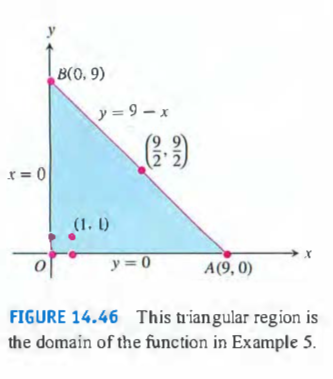
\includegraphics[scale=0.7]{m2_f9}
\end{center}

\bigskip

We must consider both interior and boundary points here. Let's start with the interior points. Finding our critical points gives
\begin{align*}
f_x &= 2-2x =0 \Rightarrow x=1\\
f_y &= 2-2y = 0 \Rightarrow y=1.
\end{align*}
So our critical point is $(1,1)$ with value $f(1,1) = 4$. We could classify it, but we don't really need to worry about it here since we are looking for absolute max and min values.

\smallskip

For the boundary points we need to consider each of the three sides of the triangle separately. Along the bottom of the triangle we know $y=0$, so we can consider our function along this line as being just a function of $x$ given by $f(x,0) = 2+2x-x^2$ on $0\leq x\leq 9$. Now since this is a function of one variable we can use techniques from Calc I to determine that this function takes max values at either the endpoints or critical points. The values at the endpoints are
\begin{align*}
f(0,0) &= 2\\
f(9,0) &= 2+18-81 = -61.
\end{align*}
The critical point(s) is $f'(x,0) = 2-2x =0 \Rightarrow x=1$. Our value here is $f(1,0) = 3.$

\smallskip

Along the side of the triangle we know $x=0$, so we can consider our function along this line as being just a function of $y$ given by $f(0,y) = 2+2y-y^2$ on $0\leq y\leq 9$. This is exactly the same situation we just dealt with, so we know the extreme values along this side are $f(0,0) = 2, f(0,9) = -61$ and $f(0,1)=3$. 

\smallskip

Finally note that along the hypotenuse of the triangle we have $y=9-x$ and we have already checked the endpoints. So we need to check the value of the function at the critical points of the function $f(x) = 2+2x+2(9-x)-x^2-(9-x)^2 = -61+18x-2x^2$. Note that $f'(x) = 18-4x = 0 \Rightarrow x=\frac{9}{2}$, giving $y=9-\frac{9}{2} = \frac{9}{2}$. Our function values here is $f(\frac{9}{2},\frac{9}{2}) = -\frac{41}{2}$.

\smallskip

To conclude we just need to pick out the largest and smallest value we found above. The maximum value was $4$ which occurred at $(1,1)$ and the minimum value was $-61$ which occurred at $(0,9)$ and $(9,0)$.
\end{example}

\newpage

% --------------------------------------------------------------
%                         Sec 14.8
% --------------------------------------------------------------

\section{Lagrange Multipliers (14.8)}

In the last section we saw how to optimize functions of two variables on unbounded and bounded regions of space. But what happens when we add a constraint to the function we want to optimize? We might think of taking the Calc I approach and solving the constraint for one of the variables, then plugging that into the function we are trying to optimize. This approach is given in the following example.

\bigskip

\hrulefill

\bigskip

\begin{example}
Find the point $P(x,y,z)$ on the plane $2x+y-z-5=0$ that is closest to the origin.

\smallskip

Here we want to find a point $P(x,y,z)$ where
\begin{align*}
|\vec{OP}| = \sqrt{x^2+y^2+z^2}
\end{align*}
is minimized and such that $2x+y-z-5=0$. First see that minimizing $|\vec{OP}|$ is the same as minimizing the function $f(x,y,z) = x^2+y^2+z^2$. Looking at the constraint, we see that we can write $z=2x+y-5$, and plugging this into $f(x,y,z)$ gives
\begin{align*}
f(x,y) = x^2+y^2+(2x+y-5)^2.
\end{align*}
Now the domain of this function $f$ is the whole $xy$-plane, so we can use techniques from the last section to solve this. Finding our critical points gives
\begin{align*}
h_x = 2x+2(2x+y-5)(2)=0, \ \ h_y = 2y+2(2x+y-5) = 0,
\end{align*}
which yields the solution $x=\frac{5}{3}, y=\frac{5}{6}$. We could then use the second derivative test to prove that this is in fact a minimizer, and then find our corresponding $z$ coordinate to be $-5/6$. This means our point closest to the origin is $P(5/3,5/6,-5/6)$. The details here are left as an exercise for the student.
\end{example}

\bigskip

\hrulefill

\bigskip

This is a good thought, but it sadly does not always go smoothly! Consider the following example.

\bigskip

\hrulefill

\bigskip

\begin{example}
Find the points on the hyperbolic cylinder $x^2-z^2-1=0$ that are closest to the origin.

\smallskip

We again want to minimize the function $f(x,y,z) = x^2+y^2+z^2$ but now our constraint is $x^2-z^2-1=0$. Solving our constraint for $z^2$ gives $z^2=x^2-1$. Plugging this back into our function $f$ gives
\begin{align*}
f(x,y) = x^2+y^2+x^2-1 = 2x^2+y^2-1.
\end{align*}
Now we again follow our process of finding critical points and get
\begin{align*}
f_x = 4x=0 \ \ \text{and} \ \ f_y = 2y=0
\end{align*}
meaning our critical point is $(0,0)$. This does not satisfy our constraint though!
\end{example}

\bigskip

\hrulefill

\bigskip

We could avoid the problem in the last example by instead solving our constraint for $x$ and using that. But there are instances where this won't work, and even if it does we do not want to be wasting time solving for certain variables that will get us nowhere. We need a new method for solving constrained optimization problems. That method is really just an application of the following theorem.

\bigskip

\begin{theorem}{(The Orthogonal Gradient Theorem)}
\\
Suppose that $f(x,y,z)$ is differentiable in a region whose interior contains a smooth curve
\begin{align*}
C: \ \bm{r}(t) = g(t)\bm{i}+h(t)\bm{j}+k(t)\bm{k}.
\end{align*}
If $P_0$ is a point on $C$ where $f$ has a local maximum or minimum relative to its values on $C$, then $\nabla f$ is orthogonal to $C$ at $P_0$.
\end{theorem}

\bigskip

We could also write this theorem for two dimensions as

\bigskip

\begin{theorem}
At the points on a smooth curve $\bm{r}(t) = g(t)\bm{i}+h(t)\bm{j}$ where a differentiable function $f(x,y)$ takes on its local maxima and minima relative to its values on the curve, $\nabla f \cdot \bm{v} = 0$, where $v=d\bm{r}/dt$.
\end{theorem}

\bigskip

\hrulefill

\bigskip

There's some nice intuition for this theorem when we consider it for functions of two dimensions. Say we are confined to walk along a single curve over some hilly landscape. As we are walking along our curve, we want to know when we reach a local maximum relative to values on the curve (i.e. we might not actually ever reach the top of a hill). In this scenario our velocity along the curve is $v$ and $\nabla f$ is the direction of steepest ascent of the landscape. If our direction of motion is \textbf{not} orthogonal to $\nabla f$, then moving farther along the curve in the direction of $\nabla f$ will get us to a higher point. It is only when $\nabla f$ and $\bm{v}$ are orthogonal that we cannot move in the direction of $\nabla f$ and reach a higher point! (You shouldn't write all of this out, I would use a picture as a guide).

\bigskip

\hrulefill

\bigskip

This theorem is the key to the method of Lagrange Multipliers. Say we want to minimize $f(x,y,z)$ subject to $g(x,y,z) = 0$. We know from the previous theorem that the local min will occur where $\nabla f$ is orthogonal to the tangent line of the level set $g(x,y,z) = 0$. We also know that $\nabla g$ is orthogonal to the curve $g(x,y,z)=0$ at every point (gradients are orthogonal to level sets). Thus we want $\nabla f$ and $\nabla g$ to be \textit{parallel}.

\bigskip

\hrulefill

\newpage

\textbf{The Method of Lagrange Multipliers}\\
Suppose that $f(x,y,z)$ and $g(x,y,z)$ are differentiable and $\nabla g \neq \bm{0}$ when $g(x,y,z) = 0$. To find the local maximum and minimum values of $f$ subject to the constraint $g(x,y,z) = 0$ (if these exist), find the value of $x$, $y$, $z$, and $\lambda$ that simultaneously satisfy the equations
\begin{align*}
\nabla f = \lambda \nabla g \ \ \text{and} \ \ g(x,y,z) = 0.
\end{align*}
These conditions are known as the \textbf{Lagrange Conditions}. For functions of two independent variables we just drop the variable $z$.

\bigskip

\hrulefill

\bigskip

\begin{example}
Find the greatest and smallest values that the function
\begin{align*}
f(x,y) = xy
\end{align*}
takes on the ellipse
\begin{align*}
\frac{x^2}{8}+\frac{y^2}{2} = 1.
\end{align*}

\bigskip

Here our function $g$ is
\begin{align*}
g(x,y) = \frac{x^2}{8}+\frac{y^2}{2} - 1.
\end{align*}
We want to satisfy our Lagrange conditions, so we need
\begin{align*}
\nabla f &= \lambda \nabla g \\ 
\Rightarrow \begin{bmatrix} y \\ x \end{bmatrix} &= \lambda \begin{bmatrix} \frac{x}{4} \\ y \end{bmatrix}\\
\text{and} \ 0&= \frac{x^2}{8}+\frac{y^2}{2} - 1
\end{align*}
or
\begin{align*}
y=\frac{\lambda}{4} x, \ \ x=\lambda y, \ \ \frac{x^2}{8}+\frac{y^2}{2} - 1=0.
\end{align*}
\end{example}
Now using the first two equations we get
\begin{align*}
y=\frac{\lambda^2}{4}y,
\end{align*}
which is true when $y=0$ or $\lambda = \pm 2$. We see immediately $y\neq 0$ since $(0,0)$ is not on the ellipse, so that means we have $x=\pm 2y$. Plugging this into $g(x,y)=0$ gives
\begin{align*}
\frac{(\pm 2 y)^2}{8}+\frac{y^2}{2} = 1 &\Rightarrow y^2+y^2=2\\
&\Rightarrow y=\pm 1.
\end{align*}
Thus $f(x,y)=xy$ takes its extreme values on the ellipse at $(\pm 2, 1)$ and $(\pm 2, -1)$. The extreme values are $f(x,y) = 2$ and $f(x,y) = -2$.

\bigskip

\hrulefill

\bigskip

\begin{example}
Find the maximum and minimum values of the function
\begin{align*}
f(x,y) = 3x+4y
\end{align*}
on the circle
\begin{align*}
x^2+y^2=1.
\end{align*}

\bigskip

Here our function $g$ is
\begin{align*}
g(x,y) = x^2+y^2 - 1.
\end{align*}
We want to satisfy our Lagrange conditions, so we need
\begin{align*}
\nabla f &= \lambda \nabla g \\ 
\Rightarrow \begin{bmatrix} 3 \\ 4 \end{bmatrix} &= \lambda \begin{bmatrix} 2x \\ 2y \end{bmatrix}\\
\text{and} \ 0&= x^2+y^2 - 1
\end{align*}
or
\begin{align*}
3=2\lambda x, \ \ 4=2\lambda y, \ \ x^2+y^2 - 1=0.
\end{align*}
\end{example}
Now using the first two equations we get
\begin{align*}
x=\frac{3}{2\lambda}, \ \ y=\frac{2}{\lambda}
\end{align*}
and plugging this into $x^2+y^2 - 1=0$ gives
\begin{align*}
\left(\frac{3}{2\lambda}\right)^2+\left(\frac{2}{\lambda}\right)^2-1&=0\\
\Rightarrow \frac{9}{4\lambda^2}+\frac{4}{\lambda^2} = 1\\
\Rightarrow 9+16=4\lambda^2\\
\Rightarrow 4\lambda^2=25\\
\Rightarrow \lambda = \pm \frac{5}{2}.
\end{align*}
This gives
\begin{align*}
x=\frac{3}{2\lambda} = \pm \frac{3}{5} \ \ \text{and} \ \ y=\frac{2}{\lambda} = \pm \frac{4}{5}.
\end{align*}
So our function $f$ takes its extreme values at $(x,y) = \pm(3/5,4/5)$. These values are $f(x,y) =5$ and $f(x,y) = -5$.

\newpage

% --------------------------------------------------------------
%                         Sec 14.8
% --------------------------------------------------------------

\section{Taylor's Formula for Two Variables}

Recall from Calc II that Taylor's formula for a function of one variable centered at $x=a$ is given by
\begin{align*}
f(x) = f(a) + f'(a)(x-a)+\frac{f''(a)}{2!}(x-a)^2+... \ .
\end{align*}
This should make Taylor's formula for two variables pretty believable.

\bigskip

\begin{definition}{(Taylor's Formula for $f(x,y)$ at the Point $(a,b)$)}
\\
Suppose $f(x,y)$ and its partial derivatives through order $n+1$ are continuous throughout an open rectangular region $R$ centered at a point $(a,b)$. Then, for all points $(x,y)$ in $R$ we have
\begin{align*}
f(x,y) &= f(a,b) + f_x(a,b)(x-a)+f_y(a,b)(y-b)+\frac{1}{2!}((x-a)^2 f_{xx}(a,b)\\
 &+2(x-a)(y-b)f_{xy}(a,b)+(y-b)^2f_{yy}(a,b) + ... + \frac{1}{(n+1)!}\left((x-a)\frac{\partial }{\partial x}+(y-b)\frac{\partial}{\partial y}\right)^{n+1}f\rvert_{(a,b)}.
\end{align*}
\end{definition}

\bigskip

\hrulefill

\bigskip

The first $n$ terms in the above formula are called the $n^{th}$ order Taylor Polynomial, and the last term is called the remainder or error. If we take an $n^{th}$ order Taylor approximation $P_n(x,y)$ of a function $f(x,y)$, we can bound the remainder term by 
\begin{align*}
|R_n(x,y)| \leq \frac{M}{(n+1)!} | |(x-a)|+|(y-b)| |^{n+1}.
\end{align*}

\bigskip

\hrulefill

\bigskip

If we are centered at $(0,0)$ this becomes

\begin{definition}{(Taylor's Formula for $f(x,y)$ at the Point $(0,0)$)}
\\
Suppose $f(x,y)$ and its partial derivatives through order $n+1$ are continuous throughout an open rectangular region $R$ centered at a point $(0,0)$. Then, for all points $(x,y)$ in $R$ we have
\begin{align*}
f(x,y) &= f(a,b) + xf_x(0,0)+yf_y(0,0)+\frac{1}{2!}(x^2 f_{xx}(0,0)\\
 &+2xyf_{xy}(0,0)+y^2f_{yy}(0,0) + ... + \frac{1}{(n+1)!}\left(x\frac{\partial }{\partial x}+y\frac{\partial}{\partial y}\right)^{n+1}f\rvert_{(0,0)}.
\end{align*}
\end{definition}

\bigskip

\hrulefill

\bigskip

\begin{example}
Find a quadratic approximation to $f(x,y) = \sin(x)\sin(y)$ near the origin.

\bigskip

In order to use Taylor's formula we will have to evaluate the function at the origin and find all partial derivatives up to second order evaluated at the origin, so we have
\begin{align*}
f(0,0) = \sin(0)\sin(0) = 0, \ \ \ &f_{xx}(0,0) = -\sin(0)\sin(0) = 0 \\
f_x(0,0) = \cos(0)\sin(0) = 0, \ \ \ &f_{xy}(0,0) = \cos(0)\cos(0) = 1\\
f_y(0,0) = \sin(0)\cos(0) = 0, \ \ \ &f_{yy}(0,0) = -\sin(0)\sin(0) = 0.
\end{align*}
So our second order approximation to this function centered at the origin is
\begin{align*}
f(x,y) \approx 0+0+0 + \frac{1}{2}\left(x^2(0)+2xy(1)+y^2(0)\right) = xy.
\end{align*}
\end{example}

\end{document}